\chapter{Monique}
``What are you getting yourself into?'' Monique wondered to herself as she knocked on the
door of the old house.

``Staying in school and refusing to fail at what I've started-that's what'' she reminded
herself as she waited. After all, what would be so bad about it? Diane had told her that this
``artist'' had been very respectful and honorable to her.

It's just so bizarre, though. Stripping to her underwear, then letting a total stranger put
a cast on her, then allowing him to take photos and make a drawing of her. What sort of person
WAS this artist, anyway?

``The sort of person who is going to help me get the bills paid this month,'' she said to
herself as the door opened.

The man who answered the door was not at all the short, bald, middle aged man she had
pictured him as. He was in his mid to late twenties, rather attractive, (or so Monique thought)
with very deep and expressive brown eyes that looked straight into hers. In fact, the only thing
about him that she had expected was his goatee.

He caught her a bit off-guard by looking her in the eye. Monique was used to men taking
stock of her attributes from the neck down before even bothering to notice if she even HAD eyes.

``I'm Monique, are you Quinn?'' She asked, hoping that this was indeed the man she was here
to see.

``Yes, please come in,'' He said opening the door for her.

``My God, this woman is beyond beautiful,'' I thought to myself as I looked at Monique. She
had long brown hair, beautifully formed facial features, and her eyes-piercing and strong, yet
revealing a softness and vulnerability that I assumed she showed to very few, if any, people.

``Please, have a seat. Would you like anything to drink?''

``Water is fine,'' she said. ``Mind if I smoke?''

``Not at all, there's an ashtray on the end table.''

In the kitchen, I dropped ice into the glasses, then filled hers with water, and mine with a
diet soda. ``Get a hold on yourself, Quinn,'' I thought. ``Be professional- she is just your
model, this is not some sort of date. She would not be here if it were not for the money. Don't
let yourself forget that, or you could wind up in serious trouble.''

After composing myself, I returned to the living room, handed her drink to her, and sat down
across from her. I tried to make some small talk, but her answer to every question was short,
almost on the edge of being impolite.

She definitely had some walls around her, this one. I didn't press the issue of getting more
comfortable with each other, as I did not want to seem inappropriate. In the end, this was
nothing more than a business arrangement, so business is what I got down to.

``So, have you ever worn a cast before?''

``No.''

``But Diane told you what it was like, I assume.''

``She said it was safe and painless, she said you were professional, and she said you pay
well.''

``Alright, do you have any questions about this whole thing?''

``Yes- when do we start, and when do I get paid?''

I couldn't help but smile. ``We start just after you get paid, and you get paid as soon as
we get into the application room.''

``I'm ready when you are.'' was her reply

I led her to the application room, and told her I would leave her alone to get ready. As I
went to retrieve the bucket, and fill it with warm water, my mind was certainly not thinking
totally straight. This woman was beautiful, exceptionally so. I've seen more than a few
beautiful women, but this one was even more beautiful than most. Her attitude, on the other
hand, was a shame. To have such exquisite beauty, with such a standoffish demeanor seemed almost
like a cruel joke. Oh well, it was only business anyway.

\begin{thought}
``Nice going- you were really a total bitch.'' Monique thought to herself as she slipped out
of her jeans. ``This guy seems nice enough. Why did you have to be so mean?'' ``Because it's a
mean world, and you have to be strong to survive, that's why,'' she muttered to herself.
Besides, what this guy is doing, no matter how nice he is, no matter how cute he is, is simply
NOT normal.'' ``Oh well, he's just making a living, trying to survive like the rest of us,'' She
thought as he came back to the room.
\end{thought}

When I returned to Monique, I almost let myself stare too long at her. In her lacy, pale
blue bra and matching underwear, she was breathtaking. In addition to the striking beauty of her
face, she had the figure to match: long, graceful, well proportioned curves, and a fabulous tan.

``As promised, payment before we start,'' I said, taking the envelope from the casting
table. She took the money from the envelope, counted it, put it back in the envelope, and then
placed it with her clothes that were neatly folded on the table by the door. As she counted the
money, I couldn't help but notice a flicker of what might have been relief in her eyes. That
expression faded as quickly as it came. She held her hands out to her side and asked ``Are you
ready?''

``Absolutely.'' I motioned to the table. ``Have a seat.''

She hopped up on the table, and asked ``So, where do we start?''

``Let's do the arm first,'' I said talking her left arm in my hands. ``Hold it out straight
for me.''

I pushed my cart to her side, and reached for the three-inch stockinette. I unrolled it, and
slid it up her arm to the armpit. I then cut it off at the end of her fingers.

``OK, now I need for you to hold your elbow at a ninety degree angle, with your thumb facing
upward.'' After she did this, I made a small slit in the stockinette over her thumb, and pulled
her thumb through. I then took a small length of one-inch stockinette, and placed it over her
thumb, positioning it straight upwards.

``Now, just hold that pose while I apply the padding.''

I wrapped two even layers of padding over her whole arm, wrist and thumb. I used two-inch
padding for the thumb and hand, and three-inch for the rest of the arm. I taped the tail of the
last roll down where it ended at her armpit. She was ready for the plaster.

I took a roll of the two-inch plaster from the cart, dipped it, and started at her wrist. I
worked the roll over her wrist, hand, and thumb. I repeated this with a second roll, then I
quickly took my scissors and trimmed the padding and stockinette back, folded it over, then
anchored everything with a third roll of two-inch plaster. I then dipped a roll of three-inch
plaster, and began where the previous plaster had stopped, working it from her wrist to just
past her elbow. Another roll followed pretty much over this same area. The next roll was used
entirely over the elbow, back and forth, to give the elbow strength. The next two rolls extended
the cast to within two inches of her armpit, and the final roll anchored the stockinette and
padding at the top, and gave some added thickness to the rest of the cast. I finished the cast
by smoothing out the plaster with my hands. I looked up at Monique.

``Is it getting warm, yet?''

``Yes, it's very warm around my thumb and hand.''

``It's not unbearable, is it?'' I asked.

``No, but it's very heavy,'' she replied.

I tapped the setting plaster with my hand, and realized that it was ready for the final
smoothing.

``Hold tight, it's not quite hard enough to rest it on anything, yet. I have a bit more
smoothing to do in the meantime.''

I took a sponge, dipped it in the water, and rubbed it over the rapidly setting plaster,
giving it a very smooth surface. This cast was turning out very nicely. After this was done, I
held the cast so that the weight on her shoulder would not be uncomfortable. I held the cast
with the palms of my hands, so as not to dent the cast and make a pressure spot. Although my
casts never live for more than a few hours, I still try to make them perfect, and above all,
comfortable.

``Is that better- with the weight?'' I asked.

``Yes, it helps,'' she said curtly.

As the plaster got warmer under my hands, I tapped the surface, and decided it was probably
safe to rest it on something. I asked her to hold it for a moment, and I retrieved a
plastic-covered pillow and a box that seemed about the right height. I placed the box beside
her, put the pillow on top of the box, and gently laid her arm on it.

``There, is that comfortable?''

``Yes.''

I rinsed my hands in the bucket, then dried them off with a towel. ``Let's take a break
before we do your leg.'' I took out my cigarettes and offered her one. ``Smoke?''

``Yes,'' she said, ``but I want one of mine. They're over with my clothes.''

I got her one of her own cigarettes, gave it to her, then lit it. (At least she let me do
THAT) I then lit one of my own for myself.

\begin{thought}
``This really doesn't feel bad at all,'' Monique thought to herself as Quinn was putting her
arm in a cast. She noticed how his hands were firm, yet gentle as he wrapped the plaster on her
arm. She found herself intently watching what he was doing. At first, she watched with
curiosity, simply wanting to see how the cast was made. Soon, however, she became fascinated by
his hands- the way she could feel them working the plaster, but how that feeling was diminishing
with each passing moment as the plaster began to set. She snapped out of her fascination when he
asked if it was getting warmer. She quickly put the enjoyment of watching him work behind her
before she answered him. She HAD to keep her distance. Still, she did have to admit to herself
that the cast looked very professional. She'd never seen a cast that went all the way to the
armpit, and covered the thumb as well. Quinn had told her over the phone that casts such as this
were actually used for certain types of injuries. The cast felt like nothing she had ever
experienced before. It was heavy, and it certainly looked hard on the outside, but it was soft
and comfortable on the inside. She tried moving her thumb inside the cast, but it would not
budge- it was held fast. She wanted to touch the outside of the cast with her other hand, but
she decided not to, since Quinn was being so careful as he touched it. If he was being careful,
maybe touching it might damage it in some way.
\end{thought}

``Well, Monique, now you can no longer say that you've never worn a cast. What do you think
of it?''

Monique quickly went back into her defensive mode. ``Well, it would suck to have to wear one
for two or three months, that's for sure. I guess it's not so bad this way, especially since I'm
being paid to wear it.''

``Damn, is money all she thinks about?'' I asked myself at her remark. I've seen this type
of woman all my life- all they care about is money, and what it buys them. What a waste- she is
so beautiful, and has no substance to back it up with. I noticed an increasing dislike for her
building inside me. ``Oh well, at least she is easy to look at. I'll try to get this next cast
done quickly, and be done with her,'' I thought to myself.

``Yes, the money does make it easier, doesn't it?'' I replied, trying to remain civil. ``The
boss does pay well.''

``Does this boss, or patron, or whatever you call him have a name?'' She asked.

``Yes, he does, but he is a public figure. He feels that if anyone ever found out about
this, it could lead to undesirable consequences for him.'' That was as much of an answer as she
needed- Hell, for all I know, she might have wanted to know so she could go find this
non-existent person, and throw herself at him- and his money, of course. With her looks, she'd
probably end up marrying money. I've seen way too many women like this in my time- they disgust
me. I snapped myself out of my contempt enough to go on.

``Well, are you ready to do your leg?'' I asked.

``Yes, if you are.''

``Then let's get started.''

I took her left leg, and rested it in the stand I had made for casting legs. The stand
rested on the floor, and had a bar going straight upwards. (Actually, it was nothing more than a
rolling stool with the seat removed) I had welded a U-shaped stirrup to the top of it, so that a
leg could rest in it. For comfort to uncasted legs, and to prevent damage to fresh casts, I had
padded the stirrup heavily. The height was adjustable, and I was very pleased with this
invention.

With her leg in the stand, I took my four-inch stockinette, and unrolled it until I was sure
there was enough to cover her leg. I held it up to her leg, and mentally figured how much extra
I would need, (stockinette tubes get shorter as they stretch in diameter) and cut it off. As I
slid the stockinette over her leg, I noticed a small scar on her knee. I guess those ``perfect''
legs aren't so perfect after all. As I slid the stockinette up to the top of her thigh, and
bunched a bit of it there, I noticed that she was watching me closely. Probably so she could
raise hell if I touched her in any inappropriate way. I was, of course, very careful not to.

I quickly worked the padding onto her leg. I used four-inch around her foot and ankle and
six-inch over the rest of it. I made sure to use my normal overlapping style of wrapping so that
she had an even two layers over the entire cast, with an extra layer at the knee and ankle. Her
leg was now ready for the plaster.

``Is your arm still alright?'' I asked her, wanting to make sure that the previous work
wasn't giving her any trouble.

``It's fine,'' she said ``The heat isn't as bad as it was.''

``Good. That means that it is pretty well set.'' I told her.

``Is it dry? Can I touch it, or try to move it?'' She asked.

``No, plaster doesn't fully set for about 24 hours,'' I answered. ``You can touch it if you
like, and you can try moving it a little bit, but don't strain against it at all- it could still
break easily. Are you ready for more of the same on this leg?''

``Sure. Go ahead''

As she explored her arm cast from both inside and out, I took a roll of four-inch plaster,
dipped it, and began wrapping it around her ankle. At first, I used a figure-eight pattern, to
hold the ankle in place, then I wrapped the entire ankle for thickness and coverage. The second
and third rolls, one on top of the other, started at her foot, and worked over her ankle, to
just slightly on her calf. I trimmed the stockinette and padding, folded it over, and anchored
it with a fourth roll of four-inch plaster. I then began working with the six-inch plaster. I
began where the four-inch left off, working the roll to just past the knee. Three more rolls
mirrored this one, then the fifth roll of six-inch plaster started just blow the knee, and ended
at mid thigh, thereby strengthening the knee. Two more rolls of six inch gave a good thickness
for her thigh, and after I had trimmed and folded the stockinette and padding, one final roll
anchored it, and gave more thickness to the thigh. I smoothed out the plaster, and after the
sponge smoothing, it was set enough at the ankle to put back in the foot rest that I had made. I
looked at my work, and I have to say, it turned out very nicely.

``Well, we need to let that dry awhile before we move you.'' I told her. ``Let me get you
your cigarettes.'' I handed her the cigarettes and lighter (she can light it herself, this time)
and asked if she needed more to drink. She agreed to a soda, and so I went to get one for each
of us.

\begin{thought}
``Pull yourself together!'' Monique thought to herself after Quinn had left the room. Her
leg tingled with the heat of the setting plaster and she had to admit she found it pleasant. She
had really been amazed, watching him work. He had been very professional, never touching her in
any inappropriate way, even though he could have done so and made it seem totally accidental.
For a brief moment, she found herself wishing he had. In the next moment, she wondered if he
might be gay. ``It doesn't matter, stupid, this is money, nothing more. What happens when you
get close to someone? You get weak, that's what happens. And what happens when you get weak? You
lose control, and then you get HURT. Just let him take his pictures, do his drawing, or whatever
it is, then get the hell out of these casts, and go save your ass with the money!'' She thought
again about the casts. It sure would be difficult trying to get through daily life with these.
She pictured herself trying to get back home while still wearing them. She smiled as she thought
to herself. ``No, not even little miss ‘I don't need anyone' could do that. Then she thought
``Bullshit- I'd find a way- I always do, don't I?''
\end{thought}

I returned to the casting room to find Monique deep in thought. ``Are you in there?'' I
asked, breaking her ``trance.''

``Yes,'' she replied instantly. She took the soda from my hand ``Thank you.''

Over the next 20 minutes, I engaged her in some forced conversation about her schooling and
activities. It wasn't a pleasant conversation, by any means, but it avoided the uncomfortable
silence that was the alternative.

She was definitely guarded, that's for sure. She didn't give me very much personal
information. Not that I wanted it, I didn't feel any desire to get to know her any more than she
appeared to want to get to know me. Of course, I'm sure, had she seen my bank statements and
stock portfolios, she would have been much friendlier. To hell with that. Not to belabor the
point, but I've seen too many like her before.

After we had let the leg cast harden for a bit, I asked her if she was ready for me to take
her into the other room for the final part of the session. She said she was ready, so I told her
how we were going to move her: I told her that I would help her stand up, then we would turn
her, and I would help her sit down in the wheelchair. I pushed the wheelchair to the side of the
table, locked the wheels, and moved the leg rests out of the way. I took her uncasted right arm,
put my other arm behind her, and helped her to stand on her uncasted right leg. We then turned,
and we sat her down in the wheelchair, smoothly and gently. I held her casted leg up with one
hand, and positioned the leg rest under it with the other. I then moved the other leg rest into
position, and she placed her foot on it.

I wheeled her into the living room, where we placed her on the couch for several photos in
different positions. I then helped her back into the wheelchair, and moved her to the window,
where we took more photos. I decided to have her standing for the sketch, so I helped her stand
up, and lean against the antique table as I drew.

The drawing was rather uninspired, given my mental state where she was concerned. I didn't
feel like I had captured the essence of her facial features very well at all. Despite this, when
I showed it to her, she said that it looked very good. As she said it, I couldn't help but
notice what seemed to be sadness in her eyes.

``If you're ready, we can get you out of these, now,'' I said.

``Definitely,'' she replied.

``Oh, you didn't like them?''

``It's not that bad,'' she answered. ``Just the same, I'm ready to have my arm and leg
back.''

I helped her back into the wheelchair, and then back to the casting room. Once she was back
on the table, I gave her my usual talk about the cast saw, and how it would not cut skin,
complete with a demonstration of my holding the humming saw to my bare hand with no injury.

I made two quick cuts, one on each side, through the plaster of each cast. I made one pass
through each cast with the bandage scissors, and the casts opened up and she was free. I left
her to get dressed.

Once dressed, she came out of the casting room.

``Thank you,'' she said in a surprisingly polite tone, maybe even a bit sad. ``This cash
will come in very handy.''

``Thank you, Monique, you're a very beautiful model, and I enjoyed working with you.'' A bit
of a lie- I admit, I stopped enjoying working with her halfway through it, but I didn't want to
be rude.

``Do you ever do repeat sittings with a model?'' She asked ``This wasn't so bad, and I
wouldn't mind maybe doing it again.''

``Well, I'm not opposed to it.'' OK, a bigger lie that time, ``But since I'm not the one
financing this, we'll have to see what the money man thinks of our work. Why don't you give me a
call in a week or two?'' What was I saying? I wanted this gold-digger gone. The words had just
come out before I knew what I was saying.

``OK, I'll be in touch,'' she said as she left.

``Whatever.'' I muttered to myself after the door closed behind her. I went to clean up the
castroom.

\begin{thought}
``Why did you say that!? Why!? Why!? You IDIOT! Monique scolded herself as she walked back
to her apartment. She went most everywhere on foot these days, since her old Firebird was long
dead of terminal transmission failure.

``Why did you ask to do it again? Why did you show that little sign of weakness?'' She
answered herself with ``Because I need the money, that's why.'' And deep down inside her, her
inner voice told her a couple of other things. Things she didn't want to hear, things she
refused to admit.
\end{thought}

\newpage
\begin{center}
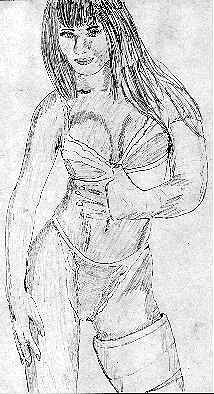
\includegraphics{images/kicks08.jpg}
\end{center}
